%\documentclass{amsart}

\documentclass{article}
\usepackage[letterpaper,hmargin=15mm,vmargin=20mm]{geometry}
\usepackage[nosetup, colorlinks]{tony}
\usepackage{graphicx}

\usepackage{amsmath,amssymb}
\usepackage{mathpazo}
\usepackage{multicol}
\usepackage{diagbox}

\usepackage{caption}% http://ctan.org/pkg/caption
\usepackage[labelformat=simple]{subcaption}% http://ctan.org/pkg/subcaption
\newcommand{\pic}[1]{\rule{#1}{#1}}% Fake picture of size #1 x #1
\renewcommand\thesubfigure{(\alph{subfigure})}% Allow sub-figure reference to be correctly printed

\usepackage{xcolor}
%\usepackage[printwatermark]{xwatermark}
%\newwatermark*[allpages,color=gray!50,angle=45,scale=3,xpos=0,ypos=0]{DRAFT}

\DeclareMathOperator{\sgn}{sgn}
\DeclareMathOperator{\NLL}{NLL}
\newcommand{\sind}[1]{^{(#1)}}

\title{6.867: Problem Set 2}
\date{October 25, 2016}

\begin{document}
\maketitle

\begin{multicols}{2}

% % % % % % % % % %
%    PROBLEM 1
% % % % % % % % % %

\section{Logistic Regression}

We implemented logistic regression with $L_2$ regularization.
Recall that the objective function for $L_2$ regularization takes the form
\begin{equation}
    E_{LR}(w, w_0) = \NLL(w, w_0) + \lambda ||w||_2^2
\end{equation}
where NLL is the logistic loss, when $y$ values are $\pm 1$:
\begin{equation}
    \text{NLL}(w, w_0) = \sum_i{\log(1+\exp(-y^{(i)}(wx^{(i)}+w_0)))}
\end{equation}
We tested our implementation against four labeled datasets,
each of size $insert$, % TODO
with two-dimesional data points $x\sind{i}$ labeled by $y\sind{i} = \pm1$.
We observed that $||w||$ decreases monotonically when $\lambda=0$,  % TODO what does this mean?
but is penalized when $\lambda=1$ (Figure~\ref{fig:weight-regularization});
indeed, regularization constrains the magnitude of $w$ [halp].  % TODO more

\begin{figure*}
   \centering
   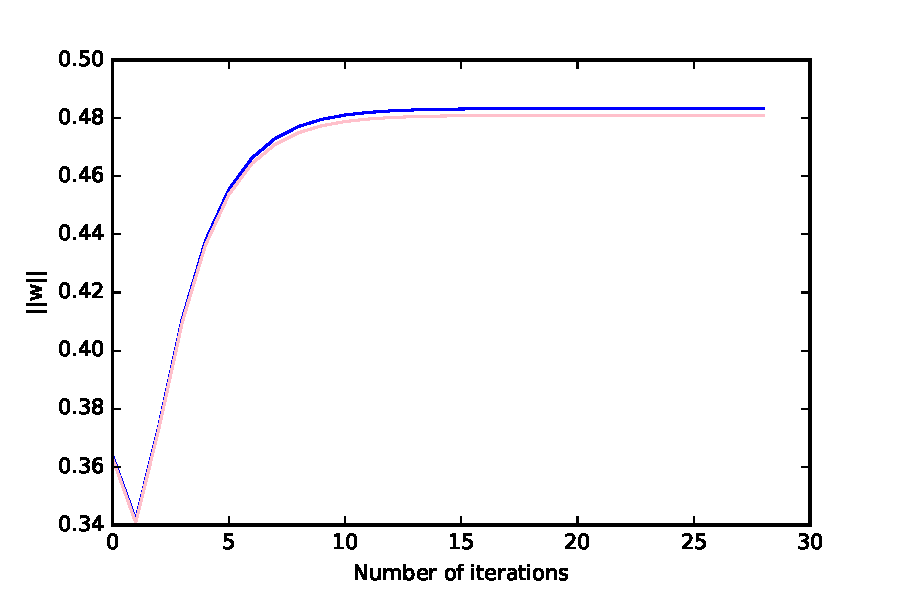
\includegraphics[width=3in]{img/1-1-weights.pdf}
   \caption{Effects of regularization on weight vector. I promise I'll replace this.}
   % TODO please replace
   \label{fig:weight-regularization}
\end{figure*}

We then compared the effects of $L_1$ and $L_2$ regularization.
Recall that the objective function with $L_1$ regularization is
\begin{equation}
    E_{LR}(w, w_0) = \NLL(w, w_0) + \lambda ||w||_1
\end{equation}
where $||w||_1 = \sum_{i=1}^n{|w_i|}$.
$L_2$ regularization generally produced
more accurate classifications as $\lambda$ increased.
Both regularization schemes produced similar decision boundaries.
For small $\lambda$,
$L_2$ regularization resulted in smaller weights
than $L_1$ regularization (figure \ref{fig:l1-l2}).

We further tested both regularization methods against four datasets (including the first),
each with similar forms of $X$ and $y$ inputs (figure \ref{fig:regularization-four}).
% TODO explain datasets
Using separate training and validation sets,
we determined the optimal regularizer and value of $\lambda$
for each dataset (table \ref{table:regularization-four}).

% TODO and then?

\begin{table*}
    \caption{Classification accuracy for logistic regression with $L_2$ and $L_1$ regularization.
    For each entry, the $L_2$ accuracy is followed by the $L_1$ accuracy.
    Also piazza says to use cross-validation / model selection stuff
    but idk what that is D: wasn't in class}
    % TODO please fix this
    \centering
    \begin{tabular}{|c||c|c|c|c|c|c|c|}
        \hline
        \backslashbox{data}{$\lambda$} & 0.125		& 0.25		 & 0.5	   & 1 & 2 & 4 & 8 \\\hline
        1	&  \color{red}1.0, 1.0 &  \color{red}1.0, 1.0 & \color{red}1.0, 1.0 &  \color{red}1.0, 1.0 &   \color{red}1.0, 1.0  & 1.0, 0.995 & 1.0, 0.995 \\
        2	& 0.805, 0.805 & 0.805, 0.805 &0.805, 0.805 & 0.805, 0.805 &  0.805,  \color{red}0.81  &  \color{red}0.81, 0.81 &  \color{red}0.81, 0.81 \\
        3	& 0.955, 0.95 & 0.96, 0.955 & 0.965, 0.955 & 0.97, 0.955 & 0.97, 0.965 &  0.97,  \color{red}0.975  & 0.97, 0.97\\
        4	& 0.4975,  \color{red}0.5 & 0.4975,  \color{red}0.5& 0.4975,  \color{red}0.5& 0.4975,  \color{red}0.5& 0.4975,  \color{red}0.5& 0.4975,  \color{red}0.5& 0.4975,  \color{red}0.5 \\\hline
    \end{tabular}
    \label{table:regularization-four}
\end{table*}
% TODO these seem to belong in two separate tables

% % % % % % % % % %
%    PROBLEM 2
% % % % % % % % % %

\section{Support Vector Machines (SVMs)}

\subsection{Dual Soft-SVM}

We implemented the dual form of soft-SVM
with third-party convex optimization software.
Recall that the soft-SVM dual optimization problem takes the form
\begin{equation}
    \label{eq:soft-svm-dual}
    \begin{array}{ll@{}ll}
        \text{maximize}  &\displaystyle -\f{1}{2}\sum_{i,j} \alpha_i \alpha_j y\sind{i} y\sind{j} \angb{x\sind{i}, x\sind{j}}
        +
        \sum_i \alpha_i \\
        \text{subject to}& 0 \le \alpha_i \le C\\
        & \displaystyle\sum_{i=1}^n \alpha_i y\sind{i} = 0
    \end{array}
\end{equation}
for training data $x\sind{i}$
labeled by $y\sind i = \pm 1$.
Hyperparameter~$C$ controls the amount of slack we permit.
Given a new data point $x$,
we predict its label $y$ as
\begin{equation}
    \label{eq:soft-svm-predict}
    y = \sgn\lt(\sum_i \alpha^*_i y\sind{i} \angb{x\sind{i}, x}\rt) \equiv \sgn(t(x))
\end{equation}
where $\alpha^*_i$ is the optimal value of $\alpha_i$
from Equation~\ref{eq:soft-svm-dual}.

For instance, given a toy dataset with positive examples
$(2, 2), (2, 3)$ and negative examples $(0, -1), (-3, -2)$,
our optimization problem takes the form
\begin{equation}
    \label{eq:soft-svm-dual-concrete}
    \begin{array}{ll@{}ll}
        \text{maximize}  &\displaystyle -\f{1}{2}\alpha^T
        \left[
            \begin{array}{cccc}
                8 & 10 & 2 & 10 \\
                10 & 13 & 3 & 12 \\
                2 & 3 & 1 & 2 \\
                10 & 12 & 2 & 13
            \end{array}
        \right]
        \alpha
        +
        \sum_{i=1}^4 \alpha_i \\
        \text{subject to}& 0 \le \alpha_i \le C\\
        & \alpha_1 + \alpha_2 = \alpha_3 + \alpha_4
    \end{array}
\end{equation}
Upon inspection,
it is clear that for large $C$
(i.e. in the hard-SVM limit),
the support vectors are $(2,2)$ and $(0,-1)$.


We tested our soft-SVM implementation
on the same four 2D datasets from the previous section.
% TODO
% makes sure 2D datasets are mentioned in previous section
Setting regularization parameter $C=1$,
we get the following support vector counts and misclassification rates on validation data:

\begin{center}
\begin{tabular}{|c|c|c|}
\hline
Dataset & Support vectors & Misclassification \\\hline
1 & 4/400 & 0/200 \\
2 & 174/400 & 36/200 \\
3 & 33/400 & 6/200 \\
4 & 392/400 & 122/400\\\hline
\end{tabular}
\end{center}

Our model clearly performs better in datasets 1 and 3.
Indeed, these datasets are linearly separable (or very nearly so),
as is apparent from Figure~\ref{fig:2-3-model-selection},
where the test data from each dataset are plotted.
Observe also that the number of support vector generally tracks the misclassification rate.

In the next section, we will kernelize our SVM routine
to handle nonlinearities in our data
(for instance, the XOR data in dataset 4 is roughly separable, but only nonlinearly).



\subsection{Kernelization}

It is often useful to map our raw data
with some nonlinear feature map $\phi$
into a higher dimensional feature space.
However, it is often infeasible to compute and store in memory
all the values $\phi(x\sind{i})$.

Therefore, we recall the ``kernel trick": the insight that
because Equation~\ref{eq:soft-svm-dual} and \ref{eq:soft-svm-predict}
only refer to values $\phi(x\sind{i})$ inside inner products
with other $\phi(x\sind{j})$,
we only need the kernel function
\begin{equation}
    k(x, x') = \angb{\phi\lt(x\rt), \phi\lt(x'\rt)},
\end{equation}
which is usually much easier to compute than the feature map $\phi$.

By replacing the inner products in
Equations~\ref{eq:soft-svm-dual} and \ref{eq:soft-svm-predict}
with the corresponding kernels,
we arrive at the kernelized soft-SVM optimization problem.
Thus, we kernelized our SVM routine
and tested it with a linear kernel
\begin{equation}
    k(x, x') = x\cdot x'
\end{equation}
and with Gaussian RBF kernels
\begin{equation}
    k(x, x') = \exp\lt(-\f{|x - x'|^2}{2\sigma^2}\rt)
\end{equation}
with bandwidths~$\sigma=0.25,0.5,1.0,2.0$ on the same four datasets as before.
We took
\[
    C \in \{0.01, 0.1, 1, 10, 100\}.
\]

In particular, we performed model selection as follows:
within both the family of linear SVMs (parametrized by $C$)
and the family of RBF SVMs (parametrized by $C$ and $\sigma$).
we took the hyperparameters that produced the best model by validation error
(using misclassification as our error metric).
Finally, we took the best of the best two models (again by validation error).
We show these best models on test data in Figure~\ref{fig:2-3-model-selection}
along with the corresponding test errors.

\begin{figure*}[t]
   \centering
   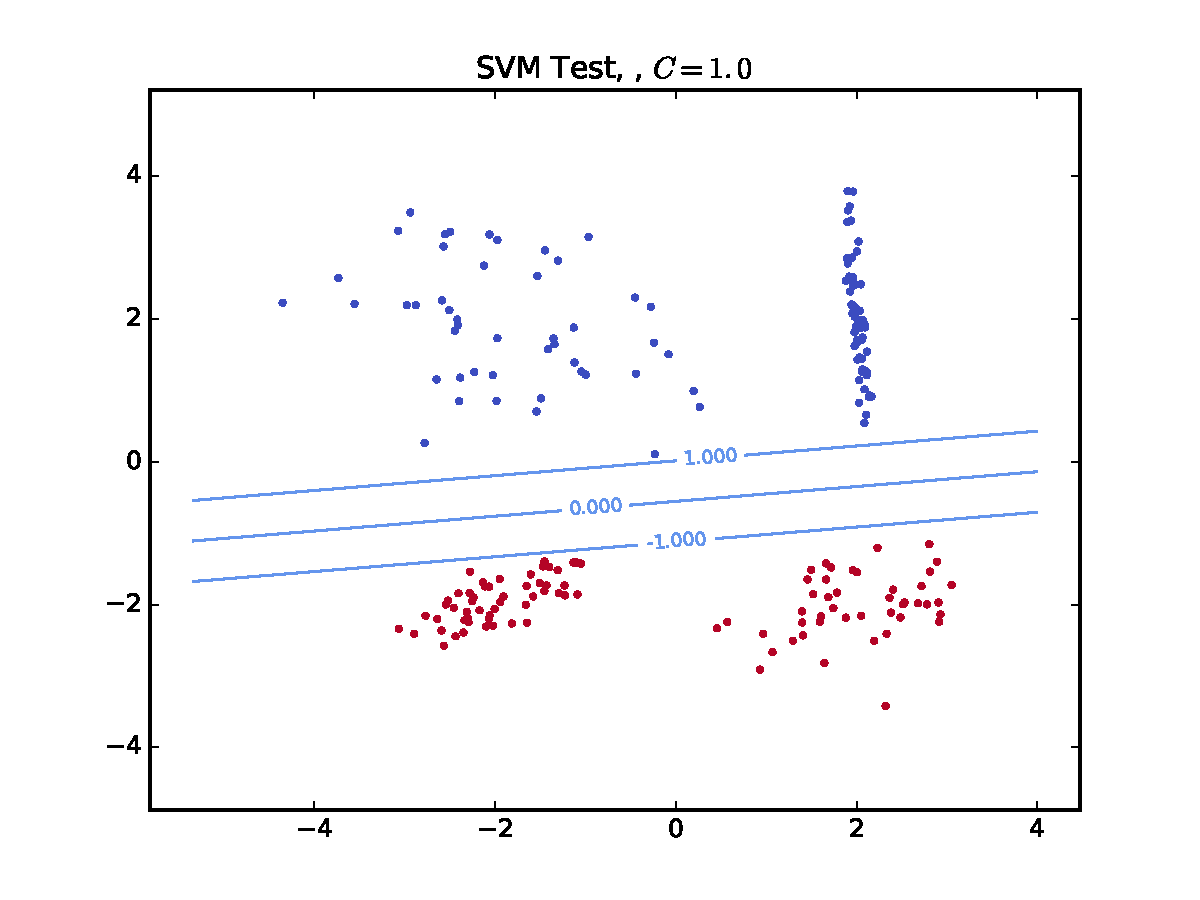
\includegraphics[width=3in]{img/p2-3-d1-c001/test.pdf}
   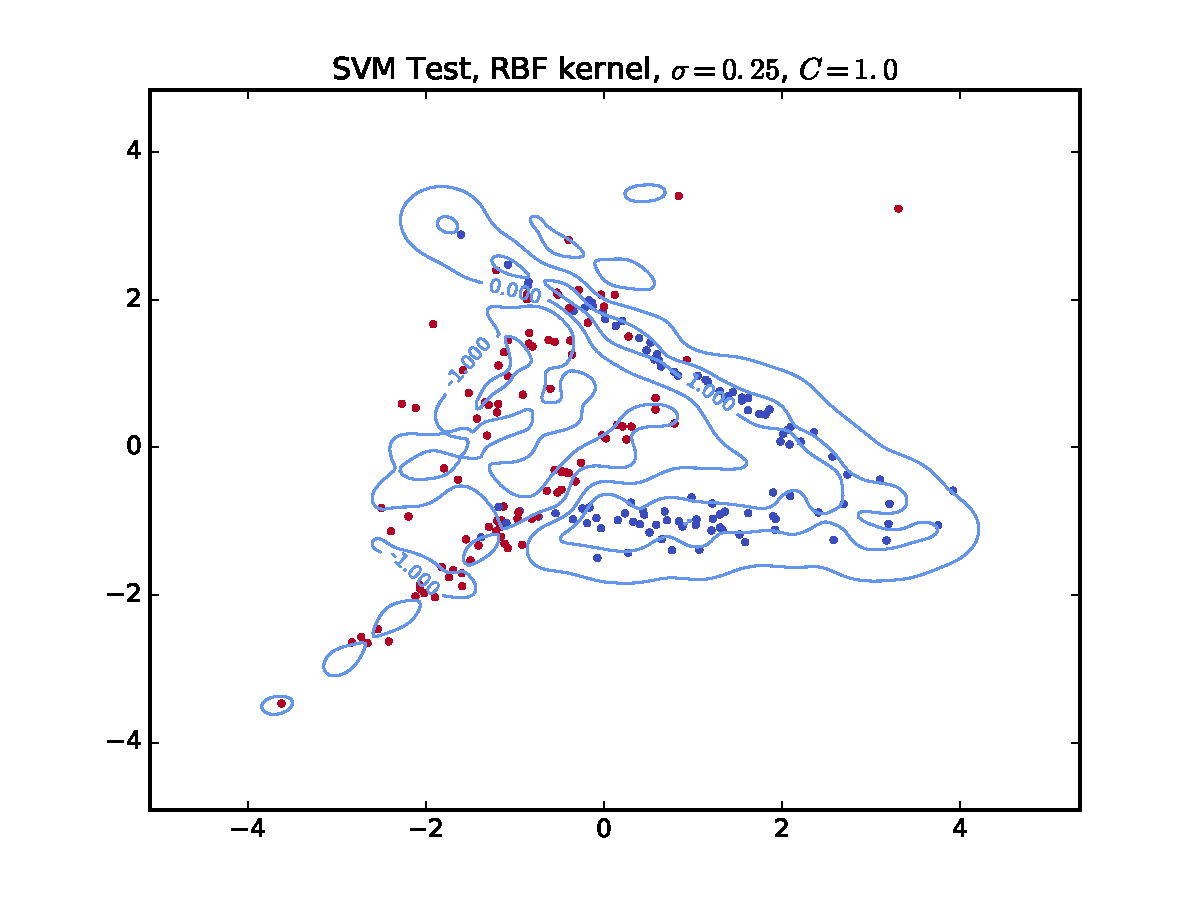
\includegraphics[width=3in]{img/p2-3-d2-c1-rbf025/test.pdf}
   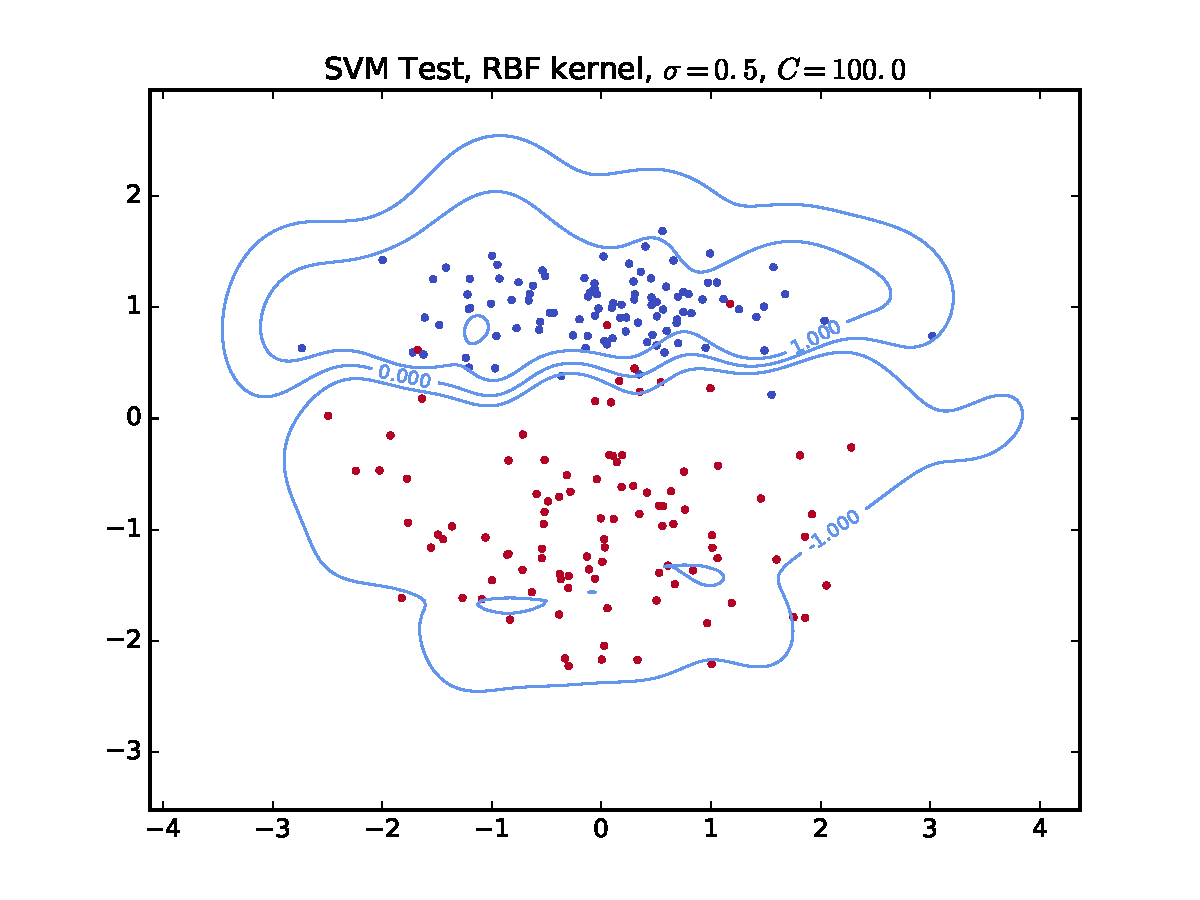
\includegraphics[width=3in]{img/p2-3-d3-c100-rbf025/test.pdf}
   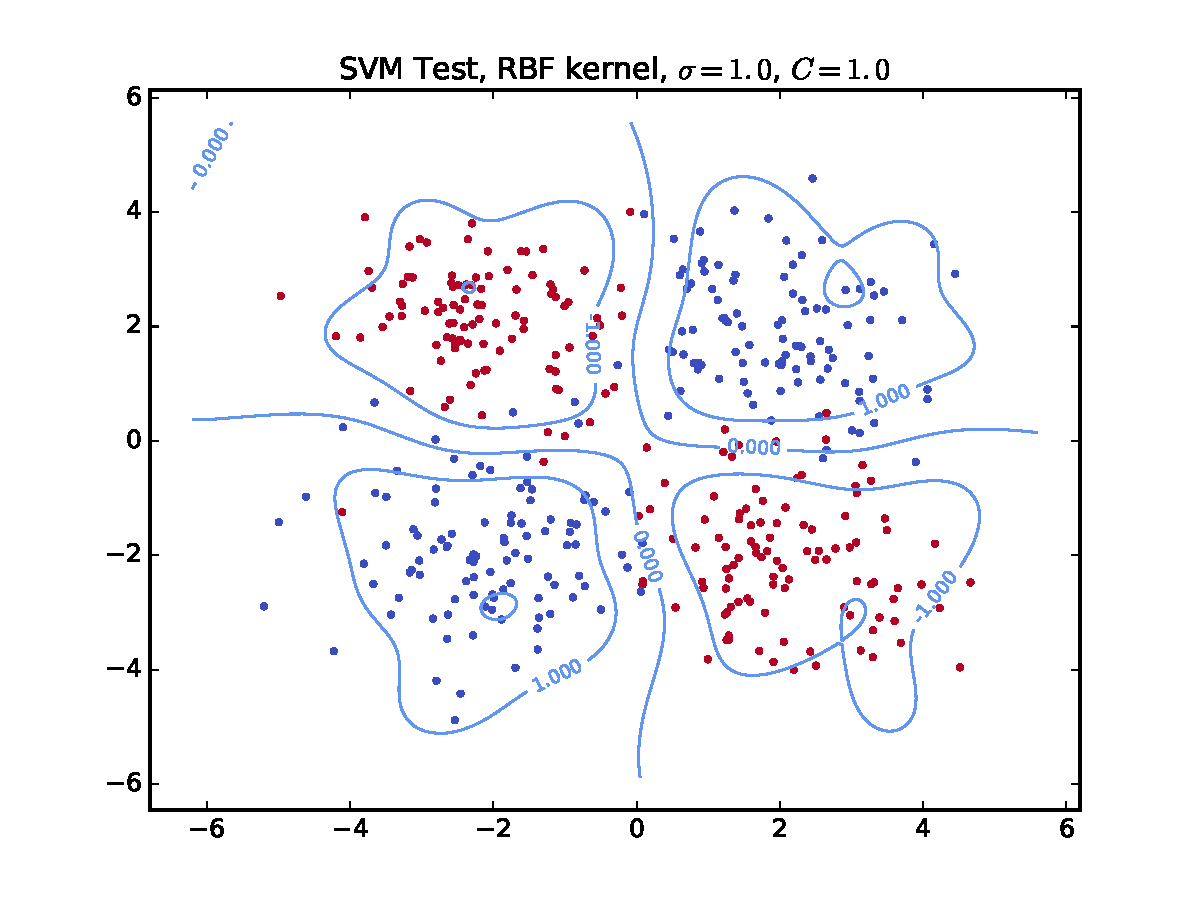
\includegraphics[width=3in]{img/p2-3-d4-c1-rbf10/test.pdf}
   \caption{Decision boundaries (with contours $t = \pm1$)
   on test data for best models produced by model selection.
   For each dataset, our best model had a misclassification rate of 0, 6, 3.5, 4.25\%, respectively.}
   \label{fig:2-3-model-selection}
\end{figure*}

In the linearly separable case, with a linear kernel,
we found that increasing $C$ led to tighter margins and fewer support vectors.
The model made no misclassifications on the validation data for $C$ in the range we tested.

Gaussian kernels worked well when we chose bandwidth~$\sigma$
commensurate to the size of the spatial features of the dataset.
Excessively small $\sigma$ created decision boundaries that overfit to training data.
On the other hand, models with $\sigma$ too large were unable to discern tight structure.
We illustrate these findings in Figure~\ref{fig:2-3-gaussian-rbf}.

In general,
Gaussian kernel SVMs have lower bias,
but potentially higher variance,
as one would expect, since using RBF kernels is equivalent to
performing mapping the raw data into an infinite-dimensional feature space.
We see this lower in bias qualitatively
in the larger number of support vectors
and in the tighter shapes of the decision boundaries.

\begin{figure*}[t]
   \centering
   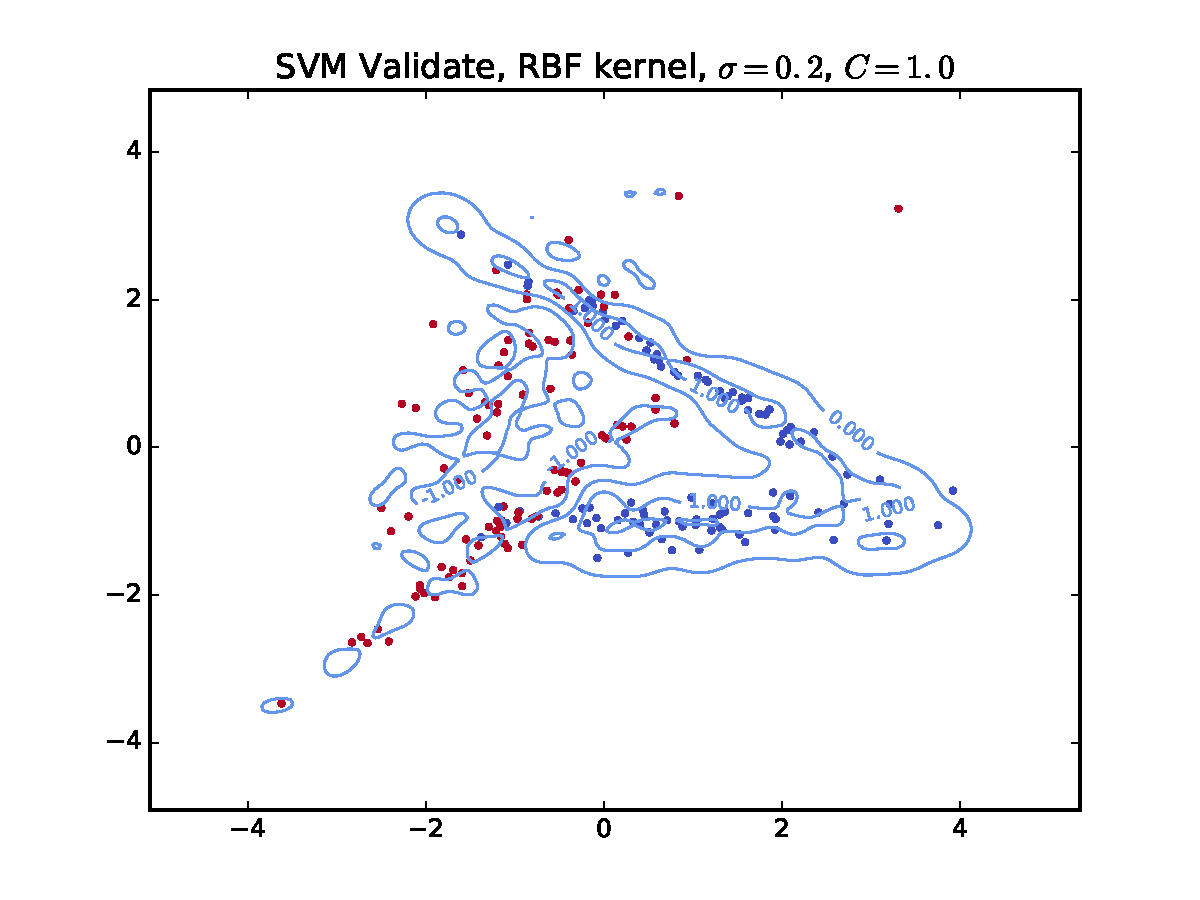
\includegraphics[width=2.4in]{img/p2-3-d2-c1-rbf02/validate.pdf}
   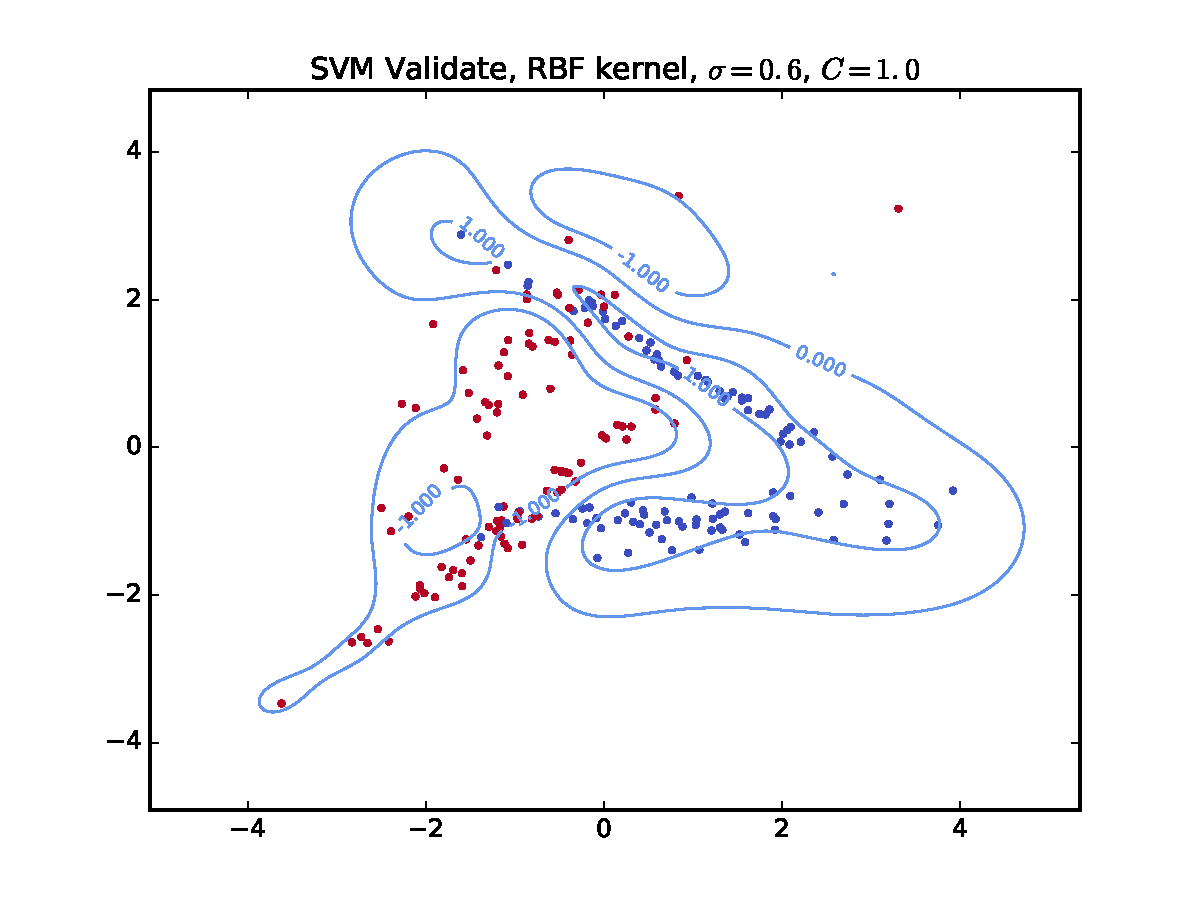
\includegraphics[width=2.4in]{img/p2-3-d2-c1-rbf06/validate.pdf}
   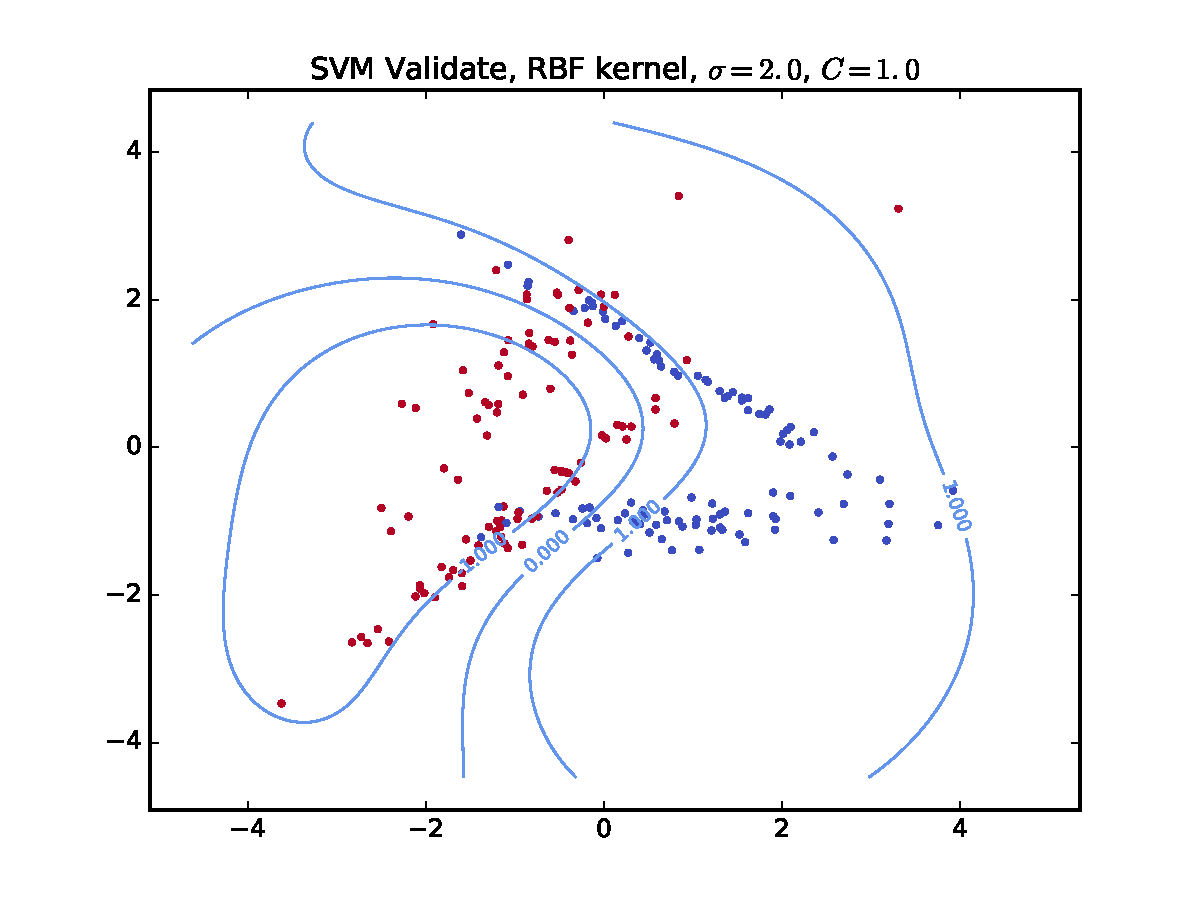
\includegraphics[width=2.4in]{img/p2-3-d2-c1-rbf20/validate.pdf}
   \caption{SVM decision boundaries (with contours $t = \pm1$) on validation data for dataset 2, with $C = 1$ and Gaussian RBF kernels with bandwidths $\sigma=0.2,0.6,2.0$, in that order.}
   \label{fig:2-3-gaussian-rbf}
\end{figure*}

We make some observations about hyperparameter~$C$.
From Equation~\ref{eq:soft-svm-dual},
larger $C$ corresponds to less tolerance for slack.
For small $C$, the model favors
maximizing the margin at the expense of slack,
so we expect increasing $C$ shrinks the geometric margin,
as our experiments confirm.
% TODO illustrate?

Consequently, there are fewer support vectors with large $C$:
the margin becomes tighter,
and the model grows increasingly averse to margin errors,
which make up the bulk of the support vectors for small $C$.

The size of the margin
is not a good metric for choosing $C$,
as can make the margin arbitrarily large
by taking $C \to 0$
(indeed, $C = 0$ allows arbitrary amounts of slack
with no penalty on the objective function).
We'd instead like a metric that evaluates
the performance of a given $C$
on unseen data.

One such metric is the hinge loss incurred
by our classifier on a validation dataset:
\begin{equation}
    \sum_{i} \max\lt(0, 1 - y\sind{i} t\lt(x\sind{i}\rt)\rt)
\end{equation}
where $t$ is the prediction function in Equation~\ref{eq:soft-svm-predict}
and where the sum is taken over all validation data.
We could also use classification error on the validation set.


% % % % % % % % % %
%    PROBLEM 3
% % % % % % % % % %

\section{SVMs with Pegasos}

While generally effective, convenient, and efficient,
SVMs become unwieldy to solve as they become large.
Thus, we may consider solving the following soft-SVM
using the Pegasos algorithm
(primal estimated sub-gradient solver for SVM):
\begin{equation}
   \min_w \lt( \f{\lambda}{2}||w||^2 + \f{1}{n}\sum_{i=1}^n{\max\{0,1-y_i(w^Tx_i)\}} \rt)
\end{equation}
The Pegasos algorithm stochastically updates our weight vector $w$ based on the following algorithm.

% TODO

We implemented Pegasos and incorporated a bias term~$w_0$ whose magnitude is not regularized.
We update $w_0$ as
\begin{equation}\label{eq:pegasos-svm}
    w_0 = w_0 + \eta_t y^{(i)}.
\end{equation}
% TODO what is \eta_t

Now recall that we define the margin as $1/||w||$. Then, as we increase $\lambda$, the margin also increases.

\begin{figure*}[h]
   \centering
	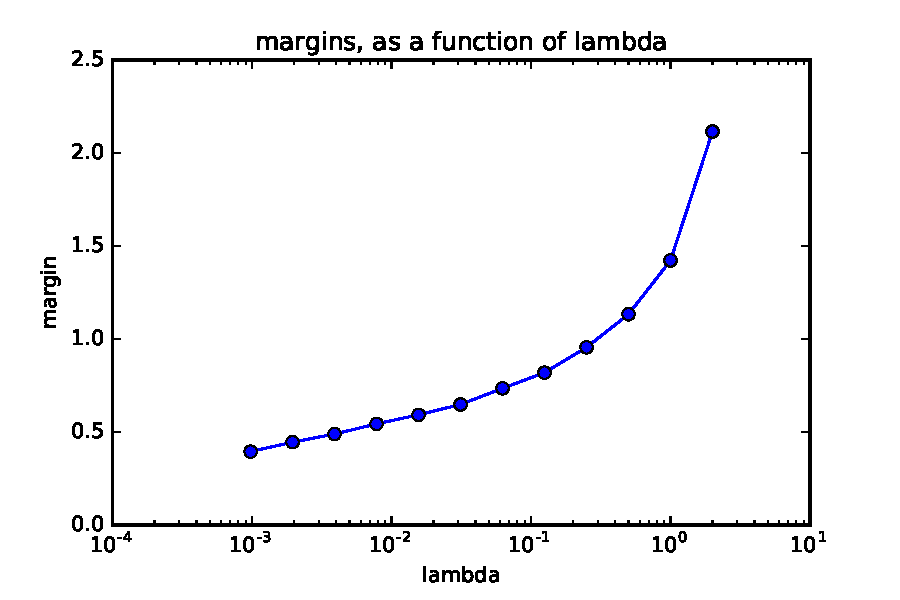
\includegraphics[width=3in]{img/3-2-margins.pdf}
   \caption{Effect of changing $\lambda$ on margins}
   \label{fig:3-2-margins}
\end{figure*}

\subsection{Kernelized Pegasos}

We can extend the Pegasos algorithm
to solve the following kernelized soft-SVM problem:
\begin{equation}
   \min_w{\f{\lambda}{2}||w||^2} + \f{1}{n}\sum_{i=1}^n{\max\{0,1-y_i(w^T\phi(x_i))\}}
\end{equation}
We implemented the following algorithm to take in a Gram matrix, where entry $k_{ij} = K(x^{(i)},x^{(j)}) = \phi(x^{(i)})\cdot\phi(x^{(j)})$.
We did not incorporate a bias term.

% TODO

Given the support vector values $\alpha$, we can make predictions for new inputs $x$ as 
\begin{equation}
    \sum_j{a_j K(x^{(i)},x^{(j)}) < 1 }
\end{equation}

% % % % % % % % % %
%    PROBLEM 4
% % % % % % % % % %

\section{MNIST Digit Recognition}

We apply these various classifiers to classify the MNIST (handwriting digit) dataset into binary subsets of digits. Each MNIST image contains 28 by 28 pixels, represented as a flattened vector of length 784. Features in this dataset take on values in the interval [0, 255] inclusive, representing the grayscale luminescence of each pixel.

We optionally normalized input pixel features to the range [-1, 1], so that an input vector $x$ is mapped to $2x/255-1$. This normalization marginally improved classification accuracy for the test set (figure \ref{fig:4-1-normalization}).

\begin{figure*}[h]
   \centering
	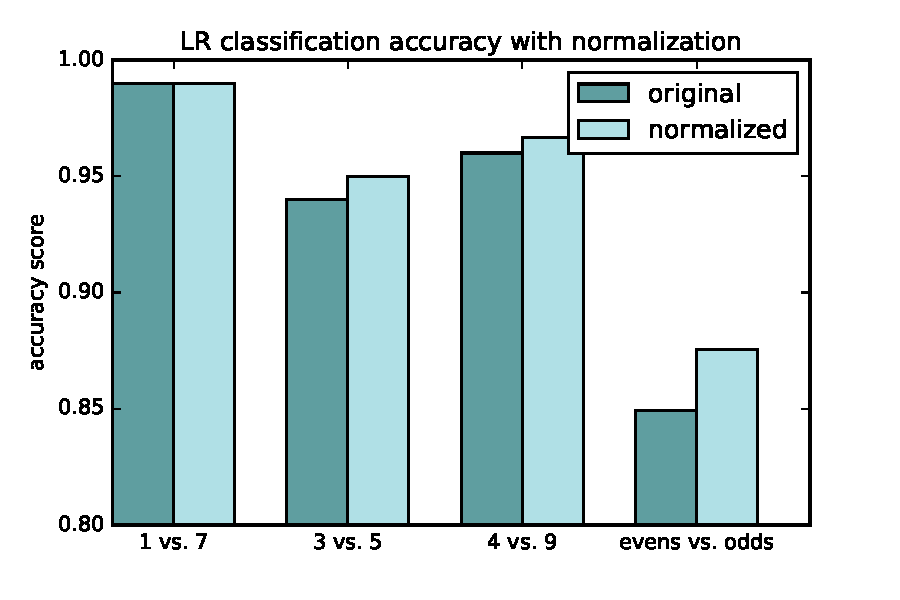
\includegraphics[width=3in]{img/4-1-normalization.pdf}
	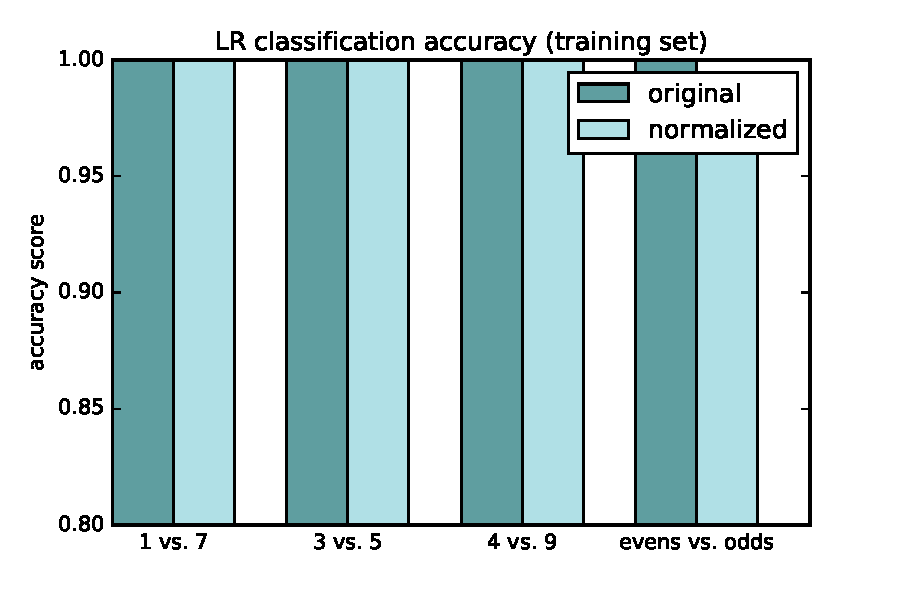
\includegraphics[width=3in]{img/4-1-normalization-train.pdf}
   \caption{Effect of pixel feature normalization on classification accuracy, for logistic regression and SVM classifiers. Will fix later}
   \label{fig:4-1-normalization}
\end{figure*}

\end{multicols}

\end{document}
